%APPENDIX A--Uncertainties ERROR ANALYSIS
\newapp

{\bf Please note:} {\em The treatment of experimental error in this
section is very brief, and is not intended to be complete!} For a more
complete treatment we strongly recommend John R.~Taylor, {\em An
Introduction to Error Analysis}, University Science Books (1997).
(The Physics Department requires this book as a text for laboratories
after the first year.  You will find copies in the libraries and at
the bookstore.) See the first four chapters in Taylor for a much more
complete discussion of the material discussed in this section.

Two other useful references that you will find in the libraries are
\begin{itemize}
\item G.\ L.\ Squires, {\em Practical Physics} (3rd edition),
Cambridge University Press (1985); and
\item D.\ C.\ Baird, {\em Experimentation: An Introduction to
Experiment and Experimental Design} (3rd edition), Prentice-Hall
(1994).
\end{itemize}

\section*{Experimental Error or Uncertainty}
%\addcontentsline{toc}{subsection}{Experimental Error or Uncertainty}
\label{scierror}

\subsection*{Meaning of Error}
     In scientific usage the word ``error" has a specialized
meaning.  It does not mean a mistake (like a miscalculation), 
but rather that some uncertainty exists in the value of
a quantity.   In this sense, errors or
uncertainties are always present in experiments.  
(The words ``error" and ``uncertainty" will be
used interchangeably here.)  While uncertainty cannot be
avoided, it must be estimated (expressed as a number) and (if possible) reduced.  
(Recall Lord Kelvin's words that opened this manual: 
``when you cannot express it in numbers, your knowledge is of a meager and
unsatisfactory kind".)   The job of estimating experimental uncertainties is
usually the most important and time-consuming part of an
experiment.  The value of an experimental result depends entirely
on an accurate estimate of its uncertainty.
%But it is possible to estimate experimental
%uncertainties, and it is important to do so if we are to
%understand how accurate or reliable an experimental result
%is --- indeed, the job of estimating experimental uncertainties is
%often the most important and time-consuming part of an
%experiment.

     All measured quantities have
errors.  Any time you report a measured quantity you should report
both the measured value, $y$, and the error $\delta y$, in the form
$y \pm \delta y$,
(e.g., 12.5 $\pm$ 0.2).  Interpret the ``$\pm$" symbol to mean that any
value between $y - \delta y$ and $y + \delta y$ is equally good.  The example
above ($y= 12.5 \pm 0.2$) should be interpreted to
mean that $y$ is quite likely to be between 12.3 and 12.7, with only
a small chance (say, 5\%) of being outside the range $12.5 \pm 0.4$.

     If we know the uncertainty in an experimental result, we can
more reasonably compare two experiments or the outcome of an
experiment with the predictions of a theory.  Two values are said
to agree if the ranges overlap.
%if they lie within their uncertainties of one another.
For example, values of $1.01 \pm 0.02$ and
$0.9 \pm 0.1$ agree; by contrast the two results $1.01 \pm 0.02$ and
$0.90 \pm 0.03$ disagree.  Or, to take another example, if a theory
predicts a value of exactly 1 and an experiment measures a value of $1.1 \pm 0.1$
(1.0 to 1.2) then the experimental result is consistent with the
theory.  Had experiment given a value of $1.10 \pm 0.01$ (1.09 to
1.11) then the experiment would have been inconsistent with the
theoretical prediction.  (Note that theory can sometimes
predict an ``errorless" value but experimental results always have
some uncertainty.)

\subsection*{Errors in Measured Quantities}

     Since the error in a measurement is as important as
the measurement itself, much of this lab course will be devoted to
teaching techniques for estimating the
error.  Note that we use the word ``estimate'' to describe the process of
finding the error. In our limited lab time there is no 
way to accurately determine experimental uncertainties.  The best we can
do is to try to find an approximate value or estimate based on our
knowledge of how the experimental results were obtained.

     There are two general types of experimental error,
{\em systematic} error and {\em random} (or statistical) error.

     A {\em systematic} error is characterized by an uncertainty that
always has the same size and sense every time you make the
measurement.  Systematic errors generally result from faulty
instrument calibration or personal bias.  For example, if the
marks on a meter stick were spaced 1.1 cm apart instead of
1 cm apart, then all distance measurements made with that meter
stick would be consistently too small.

    Systematic errors are extremely difficult to estimate.
In fact disagreements in physics
(between theory and experiment or between two experiments)
are most often resolved by discovering unexpected systematic error.
The best way to uncover systematic error is to redo the
measurement with different equipment or techniques.  In lab
we will not have time redo measurements, so we'll estimate
systematic errors by believing the calibration accuracy reported
by the equipment manufacturer.  This is a perfect example of the
wishful thinking often at the root of underestimated systematic error.
We do not recommend you follow this example in ``real life".

     By contrast, {\em random} errors are characterized by 
deviations that change in size and sign when you repeat a
measurement.  These errors may arise from changes in instrumental
operation or personal judgment.  For example, if you measured the
distance between two points twice, your first judgment of the
reading might be 1.02 cm, while the next time your reading might
be 1.03 cm.  Thus, your reading technique has an uncertainty of 0.01 cm.

     {\bf Example: } This sort of reading error can arise from parallax.  To
illustrate the parallax effect, make a zero on a sheet of paper, and
a few parallel lines on either side, like so: $|\;|\;|\;0\;|\;|\;|\;$.
Then place a pencil on the paper so the
tip is pointing at the `0' in the diagram.  Now
move your head to either side so that the pencil tip appears to
lie over one of the vertical bars.  Repeat this procedure when the indicator
pencil is raised from the paper by placing a book under it.  Now
you see for yourself that the farther away the pencil is, the
larger the possible deviation in reading the scale.



A common way to estimate 
random error is by comparing repeated observations of the
same quantity.  This technique of checking for reproducibility
can quickly yield an estimate for the random error.  For example,
if on repeated observation the values were: 1.0, 1.5, 1.2, 0.9,
0.6, then the random error seems to be about 0.5.  However if the
observations were 1.0, 2.0, 1.3, 0, 0.5, then a rough estimate
for the random error would be 1.  
Limited lab time will often force you simply guess the random error
based on the
sensitivity of the measuring device and your reading technique.  For
example, suppose you had a meter stick that had marks every 0.1
cm.  You should be able measure  to within one
half of one mark or $\pm$0.05 cm, and with care to $\pm$0.02 cm.
(Subjective differences in error estimates will occur in this lab, but you 
must be able to defend your estimate.)

     A more precise estimate of the random error depends on a
detailed understanding of statistics that is beyond the scope of
this lab manual.  (See, for example, chapter 4 in the book by
Taylor cited above.)  But we can give at least a rough idea of
what is involved.  Consider the following example:

{\bf Example:} Suppose we measure the length of an object ten times,
and obtain the values (in meters) 3.20, 3.21, 3.18, 3.17, 3.28, 3.21,
3.16, 3.24, 3.23, 3.19.  How do we estimate the uncertainty in the
length?

  We might begin by calculating the average or mean value:
\[
\langle L \rangle = {{\sum L_{i}} \over {10}} =
{{3.20 + 3.21 + 3.18 + \cdots + 3.19} \over {10}}
 = 3.2070 \mbox{ m}
\]
where $\langle L \rangle$ denotes the average value, and  $\sum L_{i}$
means first add up all the individual length
measurements (in this case the index $i$ runs from 1 to 10).

     How good is this result?  Clearly it is {\em not} good to the
four decimal places that are given!  We might begin by calculating the
{\em deviations} from the mean.  (By deviation we mean simply the
quantity $L_{i} - \langle L \rangle$.)  Consider the following table:
\begin{center}
\begin{tabular}{cccr}
 $L$ & $L_{i} - \langle L \rangle$ & $|L_{i} - \langle L \rangle|$
    & $(L_{i} - \langle L \rangle)^{2}$ \\ \hline
3.20 &  $-$.007 &       .007 &        $4.9 \times 10^{-5}$ \\
3.21 &  $+$.003 &       .003 &         $.9 \times 10^{-5}$ \\
3.18 &  $-$.027 &       .027 &       $72.9 \times 10^{-5}$ \\
3.17 &  $-$.037 &       .037 &      $136.9 \times 10^{-5}$ \\
3.28 &  $+$.073 &       .073 &      $532.9 \times 10^{-5}$ \\
3.21 &  $+$.003 &       .003 &         $.9 \times 10^{-5}$ \\
3.16 &  $-$.047 &       .047 &      $220.9 \times 10^{-5}$ \\
3.24 &  $+$.033 &       .033 &      $108.9 \times 10^{-5}$ \\
3.23 &  $+$.023 &       .023 &       $52.9 \times 10^{-5}$ \\
3.19 &  $-$.017 &       .017 &       $28.9 \times 10^{-5}$ \\
\end{tabular}
\end{center}
The second and third columns contain the deviations and the
absolute values of the deviations respectively, and the fourth
column contains the squares of the deviations.

     We might hope that the average value of the deviations will
represent the uncertainty in the length.  Note that we need to
use absolute values in our calculation of the average deviation so that the
positive and negative deviations will not cancel.  Thus we
obtain
\[
\delta L = \mbox{average deviation} = {{\sum |L_{i} - \langle L \rangle|}
  \over {10}} = {{.007 + \cdots + .017} \over {10}} = 0.027
\]
so that we can say $L = 3.21 \pm .03$ meters.  Note that the range
\[
         3.18 \leq L \leq 3.24 \;\mbox{meters}
\]
includes most but not quite all of the measurements.  This result
is to be expected --- a more advanced treatment makes it clear that
we should expect the majority (but far from all) of our values to lie within an
average deviation of the mean.

     The average deviation is hard to work with analytically,
so a more commonly used quantity is the {\em standard
deviation}, the square root of the average squared-deviation.  
Thus in our case, the standard deviation, usually
represented by $\sigma$ (the Greek letter sigma) is
\[
\sigma = \sqrt{ {{\sum (L_{i} - \langle L \rangle)^{2}} \over N}}
 = \sqrt{ {{\sum (L_{i} - \langle L \rangle)^{2}} \over {10}}}
     = 0.034 \;\mbox{m}
\]
where $N$ is the number of data points, in this case 10.

{\bf NOTE:}  A more rigorous statistical treatment would 
replace 10 by 9 in the above equation --- in general, we would
replace the number of data points $N$ by $N-1$.  See chapter 4 
in Taylor's book for
a discussion of this point.  Thus we should use
\[
\sigma = \sqrt{ {{\sum (L_{i} - \langle L \rangle)^{2}} \over {N-1}}}
 =  \sqrt{ {{\sum (L_{i} - \langle L \rangle)^{2}} \over {9}}}
     = 0.036 \;\mbox{m}
\]
Almost certainly your calculator can automatically
calculate the standard deviation of entered data; the Excel
function {\tt stdev()} reports the standard deviation of
its argument.  It will pay you to learn
how to use these functions!

Usually the average deviation is a bit
less than the standard deviation.  
Both are reasonable
estimates of the uncertainty in the measurement.  In this context
it is worth emphasizing again that we are {\em estimating}
uncertainties, not calculating exact values.

Manufacturer's spec sheets usually report an instrument's accuracy
(typically a systematic error).
It may be given as a percentage of the
reading (i.e., {\em relative} or {\em percentage}  error), an actual value (i.e., {\em absolute}
error), or a combination of the two.  For
example, let's compare two measuring devices.   Suppose the first has
a 1\%
relative error, and the second has an absolute error of $\pm$1.
If both devices read 10, then the measurement from device \#1 is
$10.0 \pm 0.1$ (1\% of 10), while that from device \#2 is $10 \pm 1$ (much
poorer).  However, if both read 1000, then the device \#1
measurement is $1000 \pm 10$ while device \#2's is $1000 \pm 1$ (much
better).

     How can we reduce errors?  In addition to the obvious
solutions like  use of more sensitive instruments
etc., we can reduce the effect of random errors (but not systematic errors)
by making repeated
measurements.  If we take $N$ measurements of the quantity
$y$, then the average value $\langle y \rangle$ of $y$ is
\[
\langle y \rangle = {{y_{1} + y_{2} + y_{3} + \cdots + y_{N}} \over
{N}}.
\]
(Note: some texts use the notation $\bar{y}$ to denote
the average value of $y$.)
Intuitively, one would expect the average value to be more accurate
than any single measurement.  Quantitatively, it turns out that we
must distinguish between

\begin{itemize}
\item {\bf standard deviation:} An estimate for the random error
($\delta y$) in any {\em single measurement} of $y$ is simply the
standard deviation:
\[
\delta y = \sigma = \sqrt{{{(y_{1} - \langle y \rangle)^{2} +
   (y_{2} - \langle y \rangle)^{2} + \cdots +(y_{N} - \langle y \rangle)^{2}}
    \over {N - 1}}}
\]

\item {\bf standard deviation of the mean:} (SDOM) The uncertainty of the
{\em average value} is given by the standard deviation
of the mean, \label{sdev.mean}


%$$\sigma_{\langle y \rangle} = \sigma / \sqrt{N},$$
\[
S = \sigma / \sqrt{N},
\]
where $N$ is the number of data points.  Note that the standard
deviation of the mean will be smaller than the standard deviation,
confirming our intuitive feeling that the average value should be more
accurate than any single measurement.
\end{itemize}

     The error estimate ($\delta y$), should always be reported along
with the measurement using the form: $y \pm \delta y$.
When  the errors in an experiment are known to be unbiased and random,
the average of repeated measurments may be of interest, in which case
you should report:
% (or
%$\langle y \rangle \pm \sigma_{\langle y \rangle}$ for
$\langle y \rangle \pm S$.

%Note: some texts use the notation $\bar{y}$ to denote
%the average value of $y$.  Using this notation the uncertainty in the average
%value is written $\sigma_{\bar{y}}$.  In certain rare instances the
%measurement may be referred to by the average value alone
%provided that the short hand notation of {\em significant figures} is
%observed.  The number of significant figures given should be only
%those digits which you are confident are approximately correct.
%For example, if the measurement is $y \pm \delta y = 21.5 \pm 0.1$ you can be
%confident that the digits 2, 1 are correct and the .5 is
%approximately correct, and you could refer to the measurement as
%21.5.  However, reporting it as either 21 or 21.50 would be
%incorrect since the former implies that the digit 1 is uncertain
%while the latter implies that the digit 5 is certain.  This
%shorthand notation is usually appropriate only in exams and on
%homework; in laboratory you should report all measured quantities
%in the form $y \pm \delta y$ unless instructed otherwise.

{\bf Important:}  {\em When you estimate the uncertainty in an experiment,
even when you do not perform repeated measurements, you are
implicitly giving a rough estimate of the standard deviation.}

\subsection*{Propagation of Error}
     Often the quantity of interest in an experiment is not
measured directly, but is calculated from other quantities that
are measured directly.  For example, to find a velocity one
measures a distance and a time interval, and divides the distance by
the
time.  In this section we will see how to find uncertainties in
{\em calculated} quantities from the known uncertainties in the
measured quantities.


\subsubsection*{High-Low Method}
\label{par:high.low.game}
Suppose we have a rectangle
for which we have measured the height $H=2.73\pm .03$~cm and the 
width $W=3.97\pm.03$~cm, and we
want to find the area.  (See Fig.~\ref{fig:rect}.)
\begin{figure}[hbt]
\begin{center}
{\resizebox{3.44in}{!}{{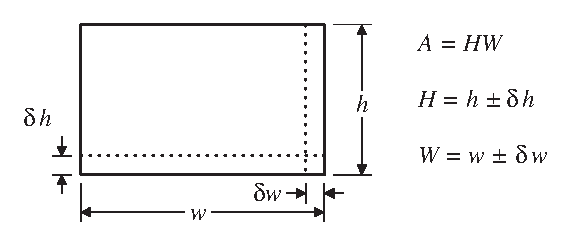
\includegraphics{figa1.eps}}}}
\end{center}
%   \centerbmp{3.72in}{1.43in}{errarea.bmp}
% \vspace{1.5in}
%  \hspace{2in}
% \special{bmp:errarea.bmp x=3.44in y=1.5in}
%\special{eps:figa1.eps x=3.44in y=1.5in}
%\special{wmf:figa1.wmf} % x=3.44in y=1.5in}
 \caption{Calculation of the area of a rectangle.  \label{fig:rect}}
\end{figure}
Clearly the best estimate for the area is $A=3.97\times2.73=10.8381\;{\rm cm^2}$.
A high estimate can be obtained by using the largest possible $W=3.97+.03=4.00$~cm
and the largest possible  $H=2.73+.03=2.76$~cm: 
$A_{\mbox{max}}=4.00\times2.76=11.04\;{\rm cm^2}$. Similarly,
a low estimate can be obtained by using the smallest possible $W=3.97-.03=3.94$~cm
and the smallest possible  $H=2.73-.03=2.70$~cm: 
$A_{\mbox{min}}=3.94\times2.70=10.638\;{\rm cm^2}$. So it seems that
$A$ must be in the range $10.638\mbox{--}11.04\;{\rm cm^2}$, which we can summarize as
$A=10.8381\pm 0.201 = 10.8\pm 0.2\;{\rm cm^2}$, where $\delta A$ was estimated
as $(A_{\mbox{max}}-A_{\mbox{min}})/2$.  We call this process of finding the
error in a calculated quantity by repeated calculation using extreme values
the ``high-low game".  It represents the crudest form of error propagation.
Some deficiencies are: (1) In a more complicated calculation, it will not clear what combination
of high and low inputs produces the extremes, so all combinations must be tested.
(2) Since the resulting error comes as the end result of a complex process, you cannot
answer important questions like: ``Which measured quantity most contributes
to the error?" or ``How much do I need to reduce the errors in the measurements to
achieve a particular accuracy in the result?".  (3) The method does not take into
account the unlikeliness of the measured quantities conspiring to achieve exactly the
right combination of extreme values to produce the extreme calculated result.

\subsubsection*{Worst-Case Formulas}
We can simplify the calculations (and solve problems (1) and (2)) by doing
the algebra for a general case.
We write the formula for the area $A$ and its uncertainty $\delta A$
as follows:
\begin{eqnarray*}
%A & = & (\ell \pm \delta \ell) \: (w \pm \delta w) \\
%  & = & \ell w  \pm \ell \: \delta w  \pm w \: \delta \ell + \delta \ell \:
%        \delta w
A \pm \delta A& = & (h \pm \delta h) \: (w \pm \delta w) \\
  & = & h w  \pm h \: \delta w  \pm w \: \delta h + \delta h \:
        \delta w
\end{eqnarray*}
An examination of the diagram should persuade you that the last
term, which is represented by the small square in the lower right-hand
corner, is much smaller than the second and third terms, represented
by the two small rectangles.  Hence to a good approximation the
best estimate for the area and its
uncertainty are given by
\begin{eqnarray*}
%\delta A = \ell \: \delta w + w \: \delta \ell
A &=& hw \\
\delta A &=& h \: \delta w + w \: \delta h
\end{eqnarray*}
where we have used the signs producing the maximum
value, so
that the uncertainties added rather than partially canceling.  Because
we have not allowed for partial cancelation, we call the resulting
error estimates ``worst-case errors".

 Note that we can also write this equation as
\begin{eqnarray*}
%\delta A & = & {{\ell w} \over {w}} \: \delta w + {{\ell w} \over {\ell}} \:
%               \delta \ell \qquad \mbox{or} \\
%\delta A & = & A \: \left({{\delta w} \over {w}} + {{\delta \ell} \over {\ell}}
%               \right)
\delta A & = & {{h w} \over {w}} \: \delta w + {{h w} \over {h}} \:
               \delta h \qquad \mbox{or} \\
\delta A & = & A \: \left({{\delta w} \over {w}} + {{\delta h} \over {h}}
               \right) \qquad \mbox{or} \\
{\delta A \over A}& = & {{\delta w} \over {w}} + {{\delta h} \over {h}}
\end{eqnarray*}
Since $\delta A/A$ is the relative error in $A$ this last equation says
that the relative error in $A$ is the sum of the relative errors in $w$ and $h$.

\subsubsection*{Usual Error Formulas}
\label{par:error.formula}
While we do not reproduce the proof here, a
more advanced statistical treatment shows that the likelihood of
partial cancelation of multiple errors (problem (3) above) can
best be addressed by using the following error estimate: 
\[
%\delta A = A \: \sqrt{ \left({{\delta w} \over {w}} \right)^{2} + \left(
%           {{\delta \ell} \over {\ell}} \right)^{2} }
\delta A = A \: \sqrt{ \left({{\delta w} \over {w}} \right)^{2} + \left(
           {{\delta h} \over {h}} \right)^{2} }
\]
In words, this equation states that the percentage error in the
area is the square root of the sum of the squares of the
percentage errors in $h$ and $w$.  %$\ell$ and $w$.

Table~\ref{table1} gives the result of this
calculation for several commonly used operations and Appendix E
provides a longer list of results.  Note that Eq.~A.2 in
that table is identical to the result we found above for the
uncertainty in the area.
It would be a useful exercise for you to confirm all of these results.

\begin{table}[ht]
\begin{center}
\caption{Formulae to calculate the error resulting from various operations.
   \label{table1}}
\vspace{12pt}
\begin{tabular}{|llll|}
\hline
 & & &   \\
{\bf Operation} & {\bf Form} & {\bf Estimated Error} & \\
 & & &   \\
\parbox{1.1in}{Addition\\
\hspace*{1ex} or Subtraction} & \parbox{.6in}{$z = x+y$ \\ $z=x-y$} &
   $\delta z = \sqrt{  (\delta x)^{2} \mathstrut+ (\delta y)^{2} } $ & (A.1) \\
 & & & \\
\parbox{1.1in}{Multiplication \\
\hspace*{1ex} or Division}& \parbox{.6in}{$z = xy$ \\ $z=x/y$} &
${\displaystyle\delta z=|z| \: \sqrt{ 
\left( { \delta x  \over x} \right)^2+
\left( { \delta y  \over y} \right)^2}}$
   & (A.2) \\
 & & &   \\
Powers & \parbox{.8in}{
$z = x^{m}\;y^{n}$\\ ${z} = x^{m}/y^{n}$} &
   $ {\displaystyle\delta z = |z| \: \sqrt{ \left (m \: {{\delta x}
\over
{x}}\right)^{2} + \left(n \: {{\delta y} \over {y}}\right)^{2} }}$ & (A.3)
\\ & & & \\
Function & 
$z = f(x)$ &
   $ {\displaystyle\delta z = \left|f'(x)\right|\; \delta x}$ & (A.4)
\\ & & & \\
\hline
\end{tabular}
\label{errorprop}
\end{center}
\end{table}

{\bf Example: }
Take a moment to look over the equations in Table~\ref{table1}.  To
illustrate how these formulas are used, we will use the distance ($S$)
and time ($t$) measurements given in Table~\ref{table2} below to find
the average velocity and the error in velocity in the interval from
$t_1$ to $t_3$.  The average velocity $v$ is given by
\[
v = {\Delta S \over {\Delta t}} = {{S_{3} - S_{1}} \over {t_{3} -
t_{1}}} .
\]

\begin{table}[ht]
\begin{center}
\begin{tabular}{|cll|}
\hline
point \# & $S$ (cm) & $t$ (sec) \\ \hline
1 & $0.00 \pm 0.05$ & $0.000 \pm 0.002$ \\
2 & $0.25$ & $0.016$ \\
3 & $0.71$ & $0.032$
\\ \hline
\end{tabular}
\end{center}
\caption{Sample distance and time data.  \label{table2}}
\end{table}

There are three steps in this calculation:  We find the error in the
numerator, then the error in the denominator, and finally, we find
the error in the velocity.

Consider the numerator.  Note that both $S_3$ and $S_1$ have
uncertainties.  Hence to find the uncertainty in
$ \Delta S = S_{3} - S_{1} = 0.71$ cm, we apply Eq.~A.1 to obtain an
uncertainty of
\[
\delta (\Delta S) = \sqrt{ (0.05)^{2} + (0.05)^{2} } = 0.07 \;
\mbox{cm} \]
To find the error in the denominator, we use the same equation.
Here $\Delta t = t_{3} - t_{1} = 0.032 \; \rm{s}$.  The uncertainty
in $\Delta t$ is
\[
\delta (\Delta t) = \sqrt{ (0.002)^{2} + (0.002)^{2} } = 0.003 \;
\mbox{s}
\]
The average velocity $v$ is
$v = 0.71/.032 \; \mbox{cm/s} = 22 \; \mbox{cm/s}$
And since we have the uncertainties in both
\[
\Delta S = 0.71 \pm 0.07 \; \rm{cm}
\]
and
\[
 \Delta t = 0.032 \pm 0.003 \; \rm{sec},
\]
we can find the error in $v = \Delta S / \Delta t$, using Eq.~A.2:
\[
\delta v = 22 \: \sqrt{ \left({{0.07} \over {0.71}}\right)^{2} +
           \left({{0.003} \over {0.032}}\right)^{2} } \; \mbox{cm/s} \:
         \approx 3 \; \mbox{cm/s}
\]
 Therefore the average velocity should be reported as $22 \pm 3$ cm/s.
Note that it would make no sense to report this result as $ 22.1875\pm 3$ cm/s;
the fractional part of the speed is of no significance if the uncertainty  is 3 cm/s.
Similarly, given the crude nature of our estimates of error, one or at most
two significant digits in the uncertainty should be reported.  
Note a fast way to lose lots of points: $ 22.1875\pm 2.99308$ --- no units and 
too many significant digits in both the number and the error.\label{appa:sigfigs}

Since the numerical value of  constants (such as
$\pi$ or $\ln(2)$) are known to very high precision, they should
be treated as error-free in calculations.  


\subsubsection*{Optional Derivation}
     In the above example the uncertainty was easy to calculate
directly.  In general, however, such will not be the case.
Therefore we will introduce a more general method of finding the
error in a calculated quantity.  The derivation involves using
calculus, and may prove difficult for beginning students to
follow in detail.  But don't give up --- what is hard for you to
understand now will seem much easier in a semester or so, when
you are farther along in your mathematics.  Until then, you can
simply use the results given in Table~\ref{table1} above.

     Consider a calculated quantity $z$ that is a function of the
measured quantities $x$ and $y$; that is, $z = z(x,y)$.  How can we
calculate $\delta z$, the uncertainty in $z$, from our measurements
$(x \pm \delta x, y \pm \delta y)$,
assuming the uncertainties $\delta x$ and $\delta y$ are random and
independent.  We begin by calculating the differential of $z$:
\[
dz = {{\partial z} \over {\partial x}} \, dx +
            {{\partial z} \over {\partial y}} \, dy
\]
(The symbol $\partial$ indicates a partial derivative---see your
calculus text if you have not yet encountered this concept.) If
the uncertainties $\delta x$ and $\delta y$ are not too large, we can
replace the differentials by the corresponding uncertainties and
write
\[
\delta z \approx \left|{{\partial z} \over {\partial x}} \, \delta x \right| +
            \left| {{\partial z} \over {\partial y}} \, \delta y \right|
\]
where we have used absolute value signs so that
uncertainties with different signs will not cancel.  This
expression gives the worst-case estimate for the uncertainty
in $z$.  A more advanced statistical treatment (allowing for partial cancelation) shows
that this expression is a bit too pessimistic, and that a better
estimate is given by taking the square root of the sum of the
squares of all the terms:
\[
\delta z \approx \sqrt{ \left({{\partial z} \over {\partial x}} \, \delta x
                 \right)^{2} + \left( {{\partial z} \over {\partial y}} \,
                 \delta y \right)^{2} }
\]
Once can derive all of the formulas in Table~\ref{table1}, as well as
the equations for more complex cases, using this technique.  See
Taylor's book, previously cited, for a more detailed treatment.

\subsection*{Uncertainties in Functional Parameters}
     We have seen how to estimate errors in measured quantities,
and in quantities calculated from those measured quantities.
However, often our goal is to find functional
relationships between measured quantities.  For example, suppose we
have a set of measurements of velocity and time that lie roughly along
a straight line.  The functional relationship between them is
therefore linear and can be written
\[
v = A + Bt
\]
where $v$ is velocity, $t$ is time, and $A$ and $B$ are constants
(here, the intercept and slope of the line).  Since the points will
not all lie exactly on the straight line, there will be a range of
possible slopes and intercepts that will all describe the data
reasonably well.  Under such circumstances, how
could we find the uncertainties in the parameters, $A$ and $B$, from
the uncertainties in $v$ and $t$?

     We will discuss this question more fully in the next three
appendices, and as usual, refer the reader to Taylor's book for a more
complete discussion.

%  The basic test that should be used in
%estimating parameter error is how much can the parameter be
%changed without changing the ability of the relationship to give
%an acceptable description of the data.  Clearly the error in
%these parameters depends on our definition of acceptable (and has
%no meaning if the fit was unacceptable to start with).  The
%errors also depend on the method of analysis and whether the
%error in the measurements have been estimated correctly.  We will
%let a computer estimate the parameter errors for more
%sophisticated functional relationships (see sections on Data Analysis,
%p.~\pageref{datanal}, and Computer Assisted Curve Fitting,
%p.~\pageref{compassis}).


